%----------------------------------------------------------------------------
\chapter{The monitoring system}
%----------------------------------------------------------------------------
\section{Goal of the implementation}

After introducing the data formats and the cyberphisical system implementation, in this part a sample application is shown that can handle connection to both data types.

The goal was to show how a connection can be created from third party applications. In further chapters the integration of the different types will be shown. The meaning of this phase is to seek for new ways to implement a web application using the connectors provided and measure the needs for such a web application. A whole test system was created to enable this.

\section{The test environment}

The system has been tested on multiple platforms. There was an Ubuntu Linux based virtual machine, which had a limited 512 MB of RAM, and a max. 10 GB storage. It's network card was hidden behind a NAT provided by the host computer. Java Runtime Environment was installed on the virtual machine for Stardog and SOS. For the web application NodeJS has been set up. 

The other platform was a Windows based computer. It had the same services (Stardog and SOS) running. The monitoring application requires NodeJs, which is a platform independent solution, so this did not mean any problem.

The chosen RDF database is Stardog Community edition. At first the software preallocates too much memory. It might be required for heavy weight applications but in our case it was not necessary.  The startup script had to be changed to make the software start. Changing this parameter does not decreases the performance significantly, compared to another computer with more memory. 

The chosen SOS server is 52north SOS 4.1 This is a recent release of the software. The used development version enables JSON communication. The server requires PostgreSQL database backend and Tomcat application server.

PostgreSQL 9.1.12 is used as the database backend for SOS. PostGIS environment had to be added. The database can be administrated using pgAdmin III from the host computer using port forward. For the Linux test environment no new users has been added, the SOS server uses the admin user to connect to the database. The database had to be created manually but tables and configuration is added during the installation automatically.

Tomcat 7 is installed to support SOS. To keep the system safe, on the Linux machine a new user is created to run the container and the application. The Stardog database is also running in a Tomcat like environment that is why it is started by the same user as the SOS server. 

\section{NodeJS: The backend of the monitoring application}

The connector application is written in JavaScript. This way the frontend and the backend application can be written using the same programming language. 
Since the V8 engine exists JavaScript can be compiled and run significantly faster\cite{v8} than before. 
The engine was introduced in 2008 and it caused a breakthrough in Javascript language. It has some new solutions that made V8 more effective, these are:
\begin{itemize}
\item \textbf{Hidden classes}: In V8 every object is a class. They are stored in a tree based structure and can be recalled faster.
\item \textbf{Dynamic Machine Code Generation}: V8 generates machine code from source without any intermediate bytecode language, like in Java.
\item \textbf{Inline cache}: It has a built in inline cache for resolving method names quicker.
\item \textbf{Efficient Garbage Collection}:Garbage collection freezes code execution and has a detailed map of the variable, however each garbage collection phase would only clear some part of the memory, it does not run full garbage collection every time.
\end{itemize}
NodeJS builds upon this V8 engine and lets JavaScript run on backend. Another advantage is that NodeJS has a single threaded, event driven core. This enables running applications faster, without worrying about thread safety. The architecture of the NodeJS environment can be seen on figure \ref{fig:node}. 
To keep the integrator separated a different user is added to run server side code on the Linux system. 
No web application container or web server is needed to run a NodeJS application. 
The software itself handles TCP connections and other modules help do it similar to Java Servlets. 
Because it has smaller overhead and dependencies, the created application should run faster than a rich Java Web application. 
NodeJS has an easy to use packaging system that makes dependency handling simple, like maven for Java. All necessary modules names are added to the related part of the package.json file and required packages are downloaded using the npm install command from a central repository. On the Windows machine a fork of NodeJS, the IOJS engine was tested. It is a community driven alternative that is fully compatible with NodeJS.
 
\begin{figure}[h]
\centering
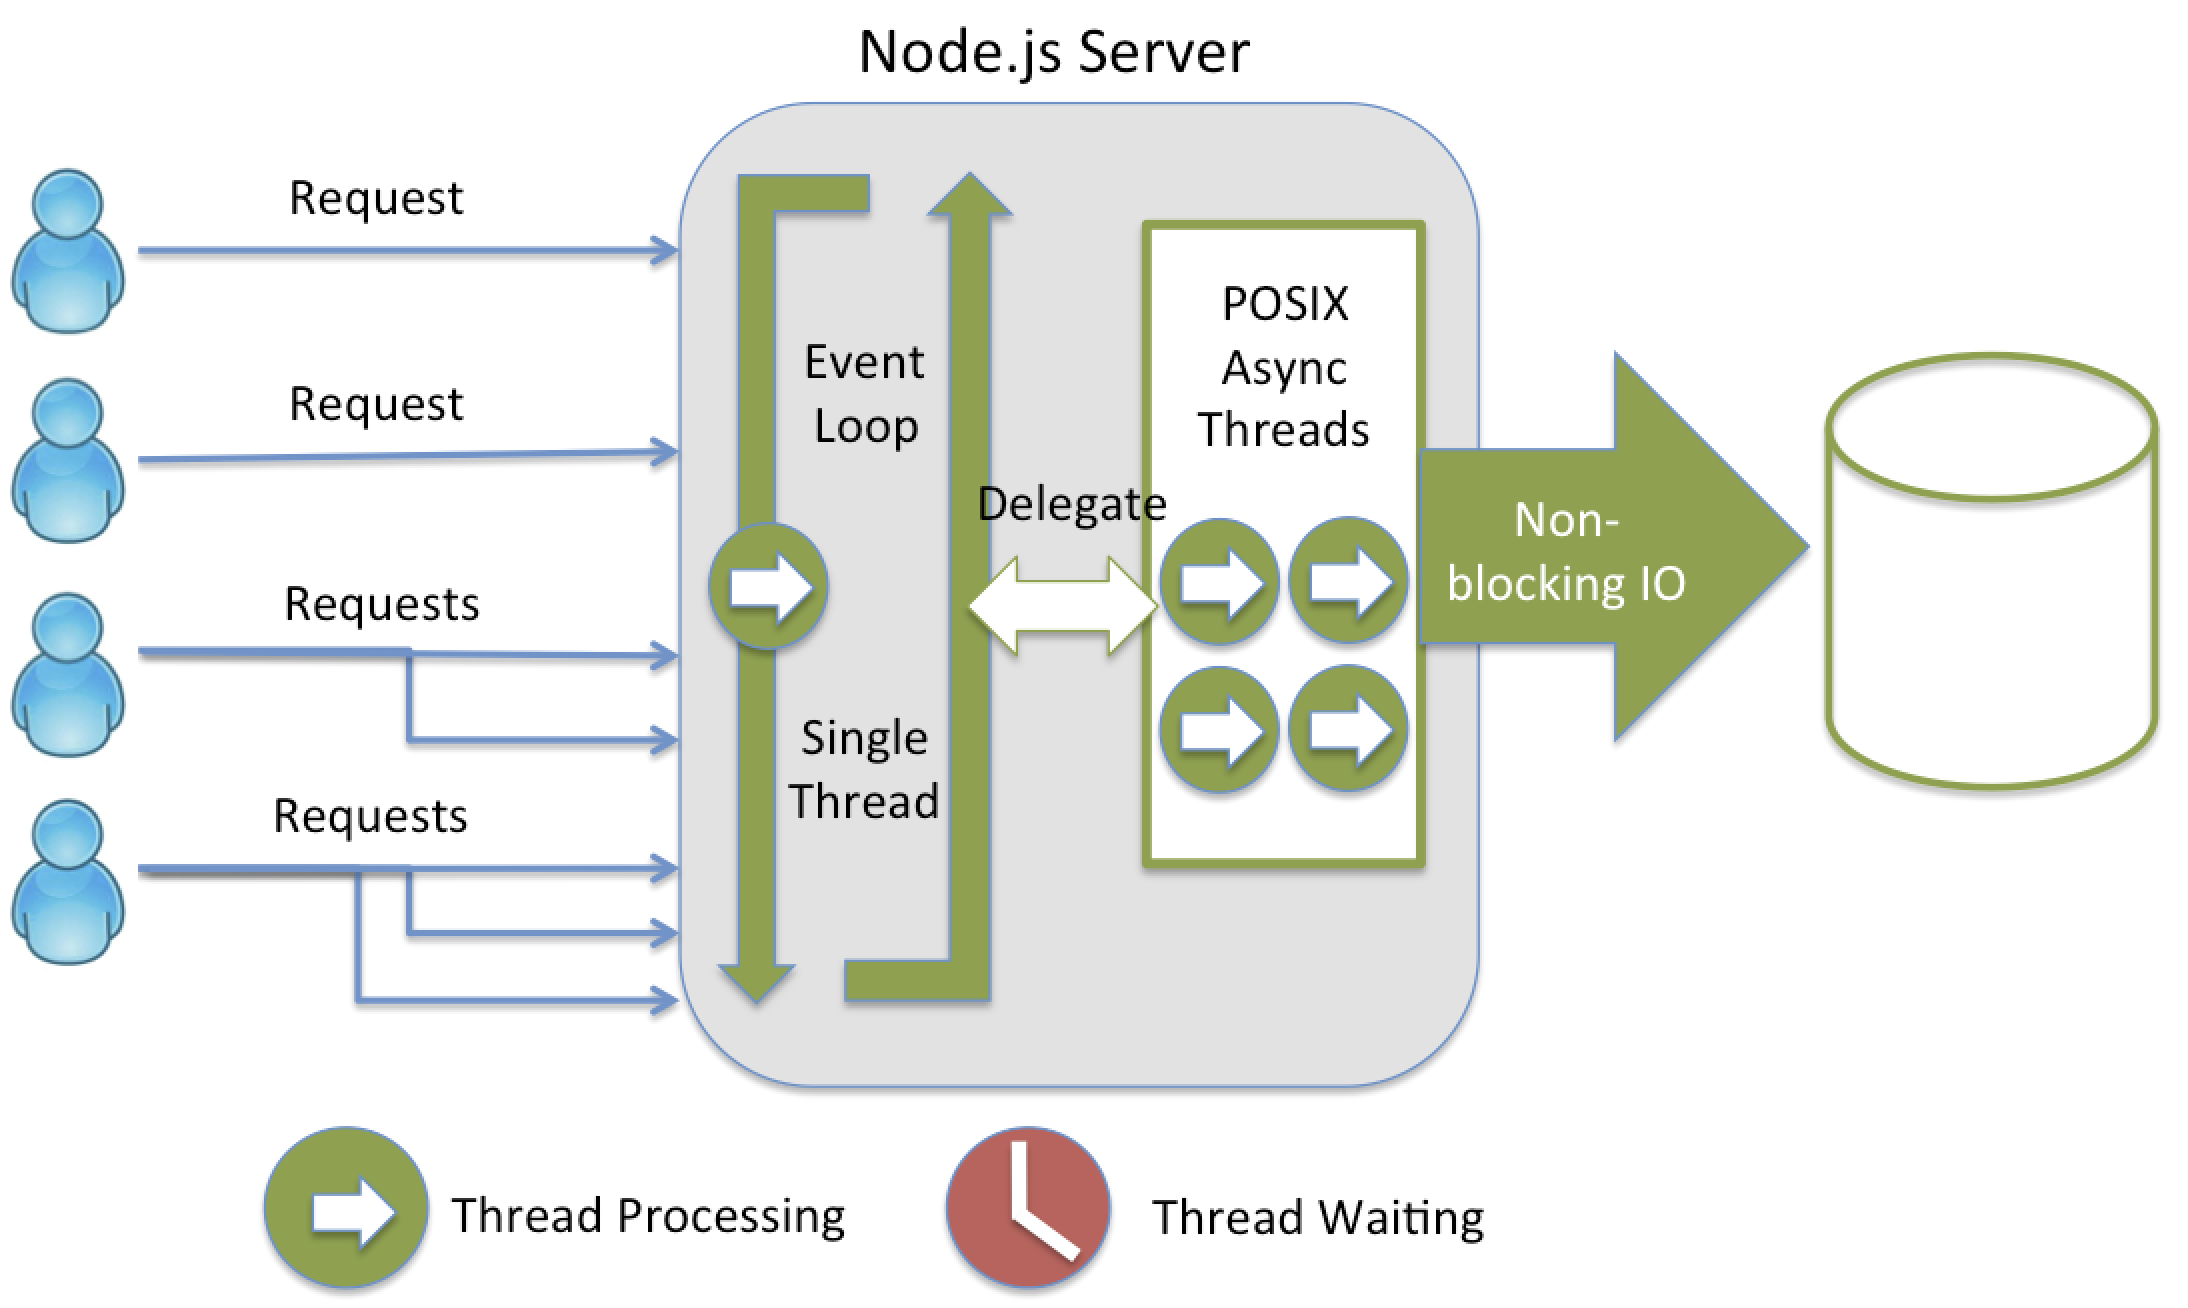
\includegraphics[width=0.6\textwidth]{figures/node.png}
\caption{NodeJS's event driven achitecture.\label{fig:node}}
\end{figure}

\section{Dependent modules}

Using the NPM (Node Package Manager) new dependent packages can be easily downloaded from a central  repository. NodeJS has a great coverage of packages, people can easily share their own modules. It contained 143 300 packages at the time of writing. In the implementation of the monitoring application there was a need for an interface for the database communication, interface for generating the web services and serving web pages. The most important packages were the following: 
\begin{itemize}

\item The ExpressJS module acts as the Servler engine for JavaScript. It handles incomming connections and parsed HTTP request are passed to a callback function which generates the responses. Different urls can have different callback functions to do routing. Express also supports many templating engines, like EJS or JADE.

\item Restler is an easy to use module that can asynchronously read a web page and parse it as JSON data and return it to the callback function. This can be used to communicate with the SOS server as it has an interface that is using JSON post requests to 
receive queries.

\item Stardog.JS is Stardog database servers own connector to get SPARQL queries. It is in early stages, however all the necessary functions are working. 

\item Nodemon, Forever or PM2 are utilities that run NodeJS codes automatically, restarts them on error or code changes. There is a support for development, that on any sourcecode change the changes are pushed to the browser without the need to refresh the browser. They can be configured to restart on error.
\end{itemize}

\section{AngularJS: the frontend of the monitoring application}

The ExpressJS module is serving the static files from the backend. The webpage itself is a single page web application which means that it consists of one html page and some partial pages that are loaded on the client side by a JavaScript framework. The framework that loads the different modules is called AngularJS. It was acquired by Google and now the project is maintained by them\cite{angular}. It's main advantage is that it implements a clear Model-View-Controller pattern. It dynamically changes the views, the HTML page based on the changes in the model, without additional coding.

\section{RDF representation of the SOS data}

The general SISRO representation was missing some data of the example use case at the time of writing. To bridge this problem the monitoring application is using a different ontology that has been created to enable sensor browsing. This ontology contains only the necessary information to query sensor information.

The first one is to create a tree on top of the sensors manually to describe the connections between each sensor. This often needs to be changed when new sensors arrive in the system. However, this tree can be exported and shared with others just like DBPedia ontologies. This can be also efficiently queried.

The second approach is to use a less redundant way by only creating rules that make sensors part of groups. These rules add a virtual groups based on the conditions defined. This is a resource intensive process that has to be re-run at every query. 

For the experiment the first way is used on a small sample ontology. The hierarchy was manually created and some properties have been added. These properties were annotated as filterable or observable. Observable meaning that the property can be seen from the monitoring system and filterable meaning that its value can be given to advance the query. The structure of the translation is not as straight forward as the created database, however it can be represented in the same way using rules. 
 
\section{Using the RDF database}

To connect to the database the Stardog.js library has been used. The statically retrieved web page asynchronously requested the list API call to get a list of the filterable properties and their range. The ranges can be either other entities, doubles, integers or strings. Depending on what the range of the property is a corresponding input box shall be rendered.

When the AJAX call responds the Angular script reloads the data with the response. 

On the backend a separate module handles the API calls, connects to the database and runst the SPARQL request. The result and additional information is returned as JSON response.

% TODO: SPARQL queries, sequence diagram, etc.

\section{Connecting the SOS server}

The JSON API can be reached easily using the Restler module to retrieve information from the SOS server. The server responds to the GetCapabilities queries with its list of the sensors and their parameters. However, yet there has not been progress in implementing the GetObservation command in the JSON interface. The JSON API is still under heavy development, thus further connection using this interface can not be done.

\section{Solving the challenge}

To solve the issue of connecting to the JSON interface there can be three different ways. 

The first one is to connect to the SOS server using another interface. There are SOAP interfaces implemented for NodeJS, by adding this layer the GetObservation method can be queried.

The second method is to implement the GetObservation method in the 52north SOS server. The development environment has been already set up, after examining the code the changes shoul be made easily. 

Because of the many changes that are needed to display SOS data changing to an existing SOS client should be a great step forward. The existing client can be extended by semantic functions using the Stardog library provided and the some SPARQL queries. The development environment for the SWE Client is also ready to use.

\section{Using the Software}

Thanks to NodeJS package management the software is easy to deploy. After installing NodeJS - in Windows there is a straight-forward installer, for Ubuntu it can be easily installed using apt - the git project has to be cloned to the server. In the project directory (sensormonitor)  the npm install command installs the missing modules and the npm start command starts the application with Nodemon. The url of the rdf database can be changed in rdf\_parser.js. The installation commands are shown on listing \ref{lst:install}

\begin{lstlisting}[caption={Install steps for the software\label{lst:install}}]
#0. install NodeJS and npm
sudo apt-get install nodejs
#1. clone the project to your destination
git clone --depth 1 https://djlancelot@bitbucket.org/djlancelot/sensormonitor.git
#2. change into project folder
cd sensormonitor
#3. install missing dependencies
npm install
#4. start the application
npm start
\end{lstlisting}